\documentclass{beamer}
\usetheme{Warsaw}

\usecolortheme[rgb={0.2,0.4,1}]{structure}
\definecolor{grayColor}{rgb}{0.255,0.25,0.275}
\setbeamercolor{section in head/foot}{bg=grayColor,fg=white}
\setbeamerfont{subsection in head/foot}{size=\small}

\usepackage{multimedia}
\usepackage[T1]{fontenc}
\usepackage[utf8]{inputenc}
\setbeamertemplate{footline}[frame number]{}
\setbeamertemplate{navigation symbols}{}

\title{Défier l'ordinateur au Sokoban}
\author{Aymeric BEAUCHAMP\\Dimitri CHAGNEUX\\Valentin LEBLOND\\Baptiste MORI}
\date{Avril 2018}

\begin{document} 
\maketitle 

\frame{\tableofcontents}

\section{Notre projet}

\subsection{Objectifs}
\begin{frame}
\begin{itemize}
\item Programmer le jeu Sokoban
\item Ajout d'une interface graphique
\item Résolution automatique de niveau
\item Jouer contre l'ordinateur en temps réel
\end{itemize}
\end{frame}

\subsection{Présentation du sokoban}
\begin{frame} % premier transparent
\begin{columns}
\hspace{0.5cm}
\begin{column}{5cm}
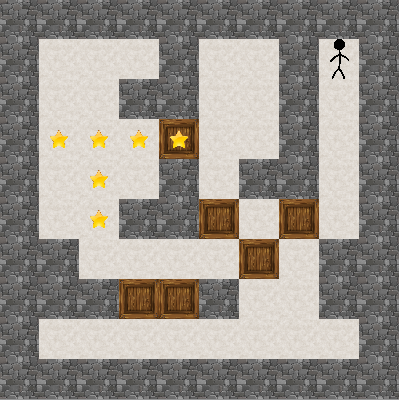
\includegraphics[scale=0.3]{images/sokoban.png}
\end{column}
\begin{column}{6cm}
\begin{itemize}
\item Jeu de réflexion (puzzle)
\item Poussée de caisses
\item Objectif : ranger toutes les caisses 
\end{itemize}
\end{column}
\end{columns}
\end{frame}

\subsection{Organisation du projet}
\begin{frame}
\begin{itemize}
\item 1ère séance : conception structure projet + début
\item Puis, 3 groupes :
\begin{enumerate}
\item Version console, gestion de sauvegarde/chargement de fichiers
\item Solveur
\item Interface graphique
\end{enumerate}
\item Décalage entre version console et version graphique
\item Rassemblement pour la finalisation
\end{itemize}
\end{frame}

\section{Architecture du projet}
\begin{frame}
Architecture du projet
\end{frame}

\section{Eléments techniques}
\subsection{Deadlocks}

\begin{frame}

\begin{block}{Définition}
Une caisse en deadlock, est une caisse qu'on ne peut plus déplacer directement ou indirectement. Le jeu est donc bloqué.
\end{block}
\vspace{0.5cm}
\begin{center}
\begin{columns}
\begin{column}{4cm}
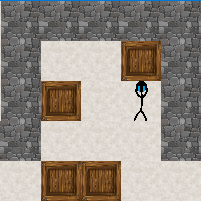
\includegraphics[scale=0.7]{images/deadlock1.PNG}
\end{column}
\begin{column}{4cm}
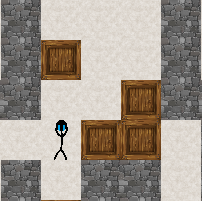
\includegraphics[scale=0.7]{images/deadlock2.PNG}
\end{column}
\end{columns}
\end{center}
\end{frame}

\subsection{Solveur}
\begin{frame}
\frametitle{Démonstration}
\movie[autostart]{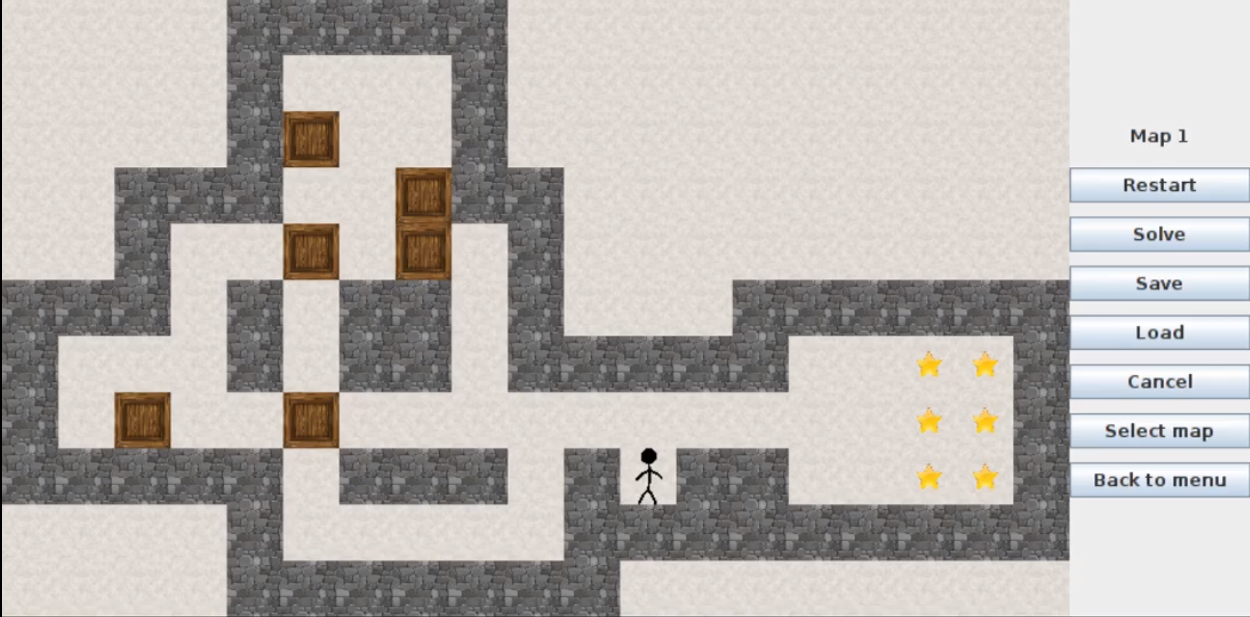
\includegraphics[scale=0.25]{images/im_solver.png}}{images/solveur.flv}
\end{frame}


\section{Expérimentations et usages}
\begin{frame}
Expérimentations et usages
\end{frame}

\section{Conclusion}
\subsection{Réalisation des objectifs}
\begin{frame}
\begin{itemize}
\item Globalement les objectifs ont été réalisés
\item Première expérience de conception logicielle
\item Travail en groupe 
\end{itemize}
\end{frame}

\subsection{Améliorations possibles}
\begin{frame}
\begin{itemize}
\item Solveur
\begin{itemize}
\item Réduire la mémoire utilisée
\item Trouver de meilleurs chemins
\end{itemize}
\item Meilleur comportement de l'ordinateur en mode \textit{anytime}
\item Ajouter des fonctionnalité de terrain (par exemple des téléporteurs,etc.)
\item Statistiques (temps de résolution, nombre de coups)
\end{itemize}
\end{frame}


\end{document}
